% $Id: ArchitectureIntro.tex,v 1.1 2008/01/31 18:04:16 dconway Exp $
\chapter{\label{chapter:Introduction}Introduction}

\chapauthor{Darrel J. Conway}{Thinking Systems, Inc.}

Early in 2002, Goddard Space Flight Center (GSFC) began to identify requirements for the flight
dynamics software needed to fly upcoming missions that use formations of spacecraft to collect data.
 These requirements ranged from low level modeling features to large scale interoperability
requirements.  In 2003 we began work on a system designed to meet these requirements; this
system is GMAT.

The General Mission Analysis Tool (GMAT) is a general purpose flight dynamics modeling tool built on
open source principles. The GMAT code is written in C++, and uses modern C++ constructs extensively.
GMAT can be run through either a fully functional Graphical User Interface (GUI) or as a command
line program with minimal user feedback. The system is built and runs on Microsoft Windows, Linux,
and Macintosh OS X platforms. The GMAT GUI is written using wxWidgets, a cross platform library of
components that streamlines the development and extension of the user interface.

Flight dynamics modeling is performed in GMAT by building components that represent the players in
the analysis problem that is being modeled.  These components interact through the sequential
execution of instructions, embodied in the GMAT Mission Sequence. A typical Mission Sequence will
model the trajectories of a set of spacecraft evolving over time, calculating relevant parameters
during this propagation, and maneuvering individual spacecraft to maintain a set of mission
constraints as established by the mission analyst.

All of the elements used in GMAT for mission analysis can be viewed in the GMAT GUI or through a
custom scripting language. Analysis problems modeled in GMAT are saved as script files, and these
files can be read into GMAT. When a script is read into the GMAT GUI, the corresponding user
interface elements are constructed in the GMAT GUI.

The GMAT system was developed from the ground up to run in a platform agnostic environment.  The
source code compiles on numerous different platforms, and is regularly exercised running on
Windows, Linux, and Macintosh computers by the development and analysis teams working on the
project.  The system can be run using either a graphical user interface, written using the open
source wxWidgets framework, or from a text console.

The GMAT source code was written using open source tools.  GSFC has released the code using the
NASA open source license.

\section{The Tool}

Figure \ref{DLS_Sample} shows a sample run using GMAT on Windows XP.  GMAT can be run using either a
custom scripting language or components configured directly from the user interface.  GMAT scripting
is designed to run either from within GMAT, or from inside of the MATLAB product from MathWorks.

\begin{figure}
\begin{center}
%  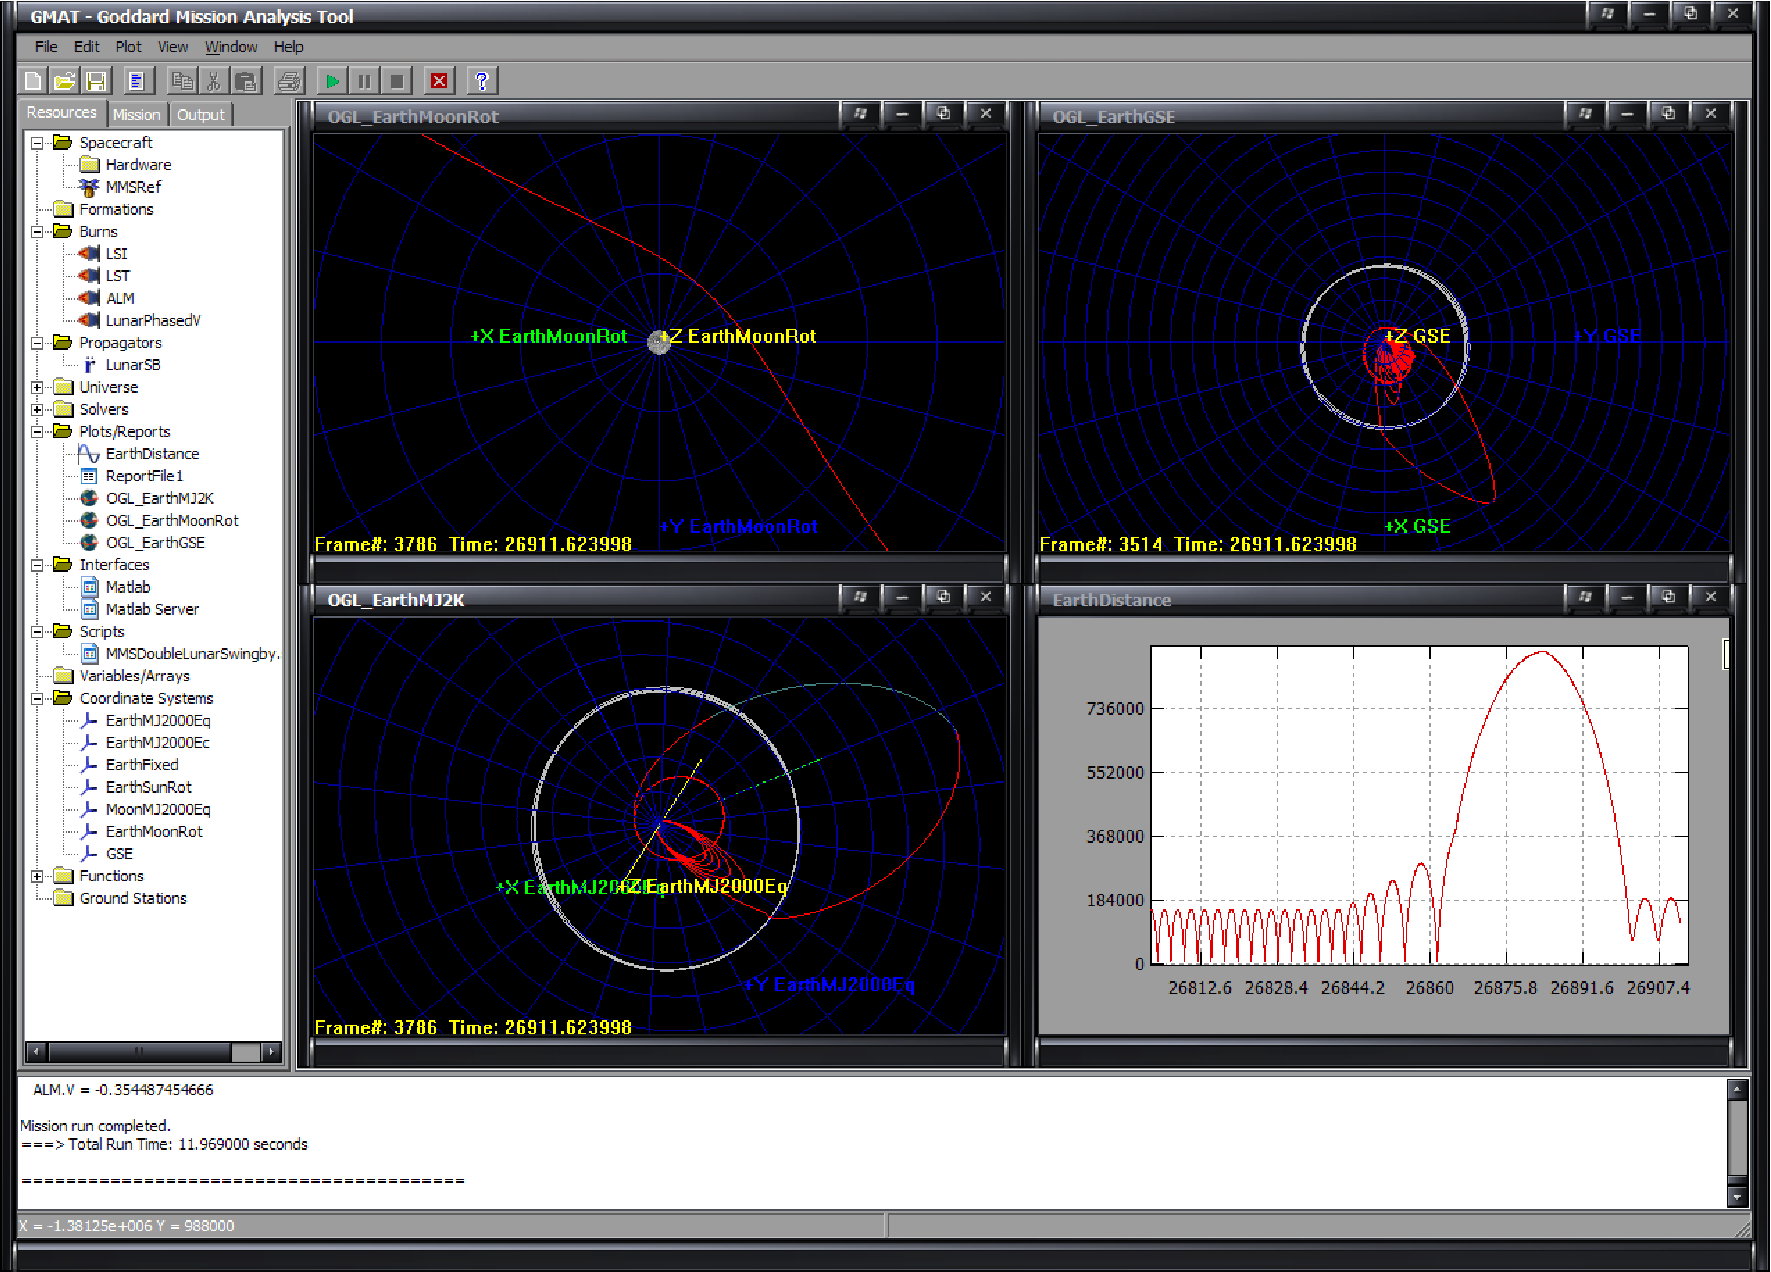
\includegraphics[width=\textwidth]{Images/DoubleLunarSwingby.png}
  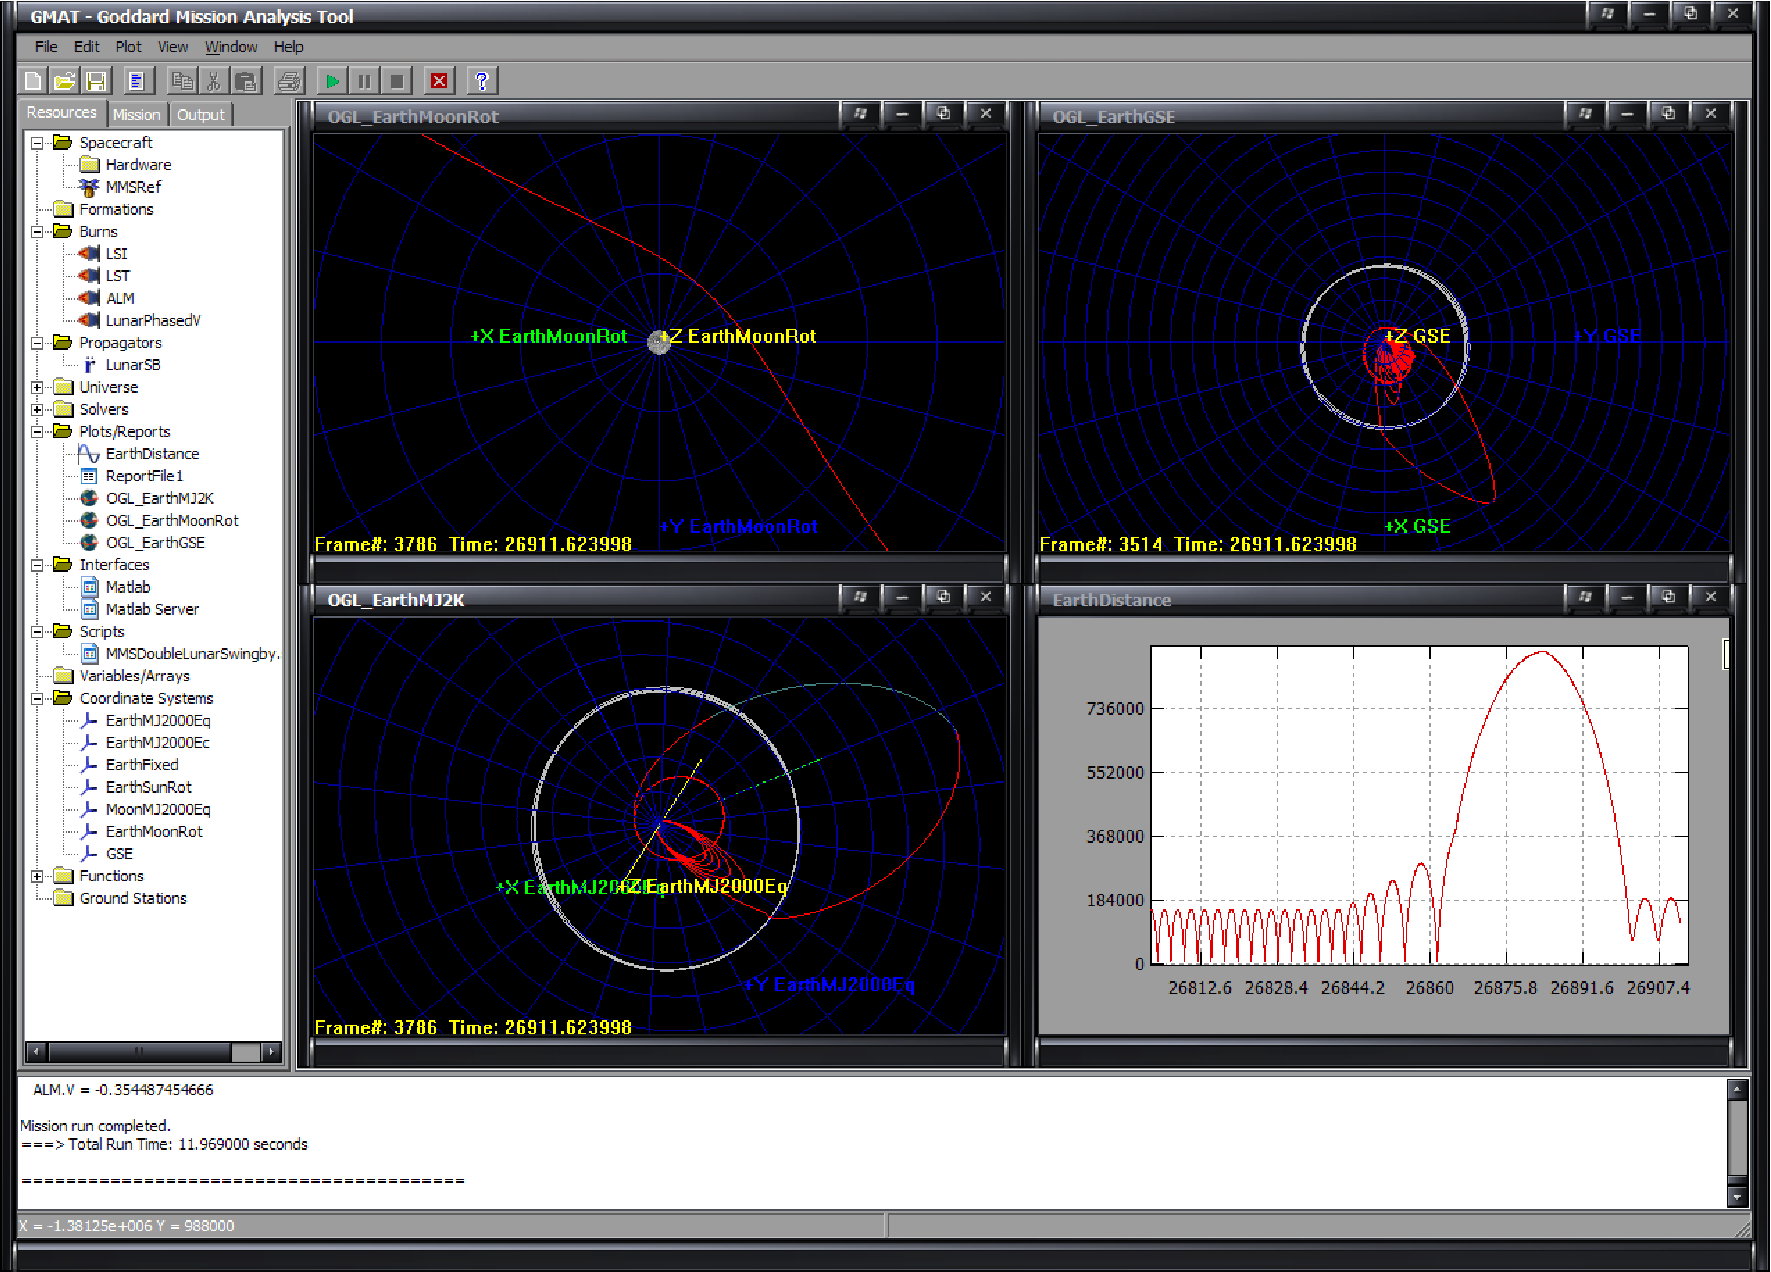
\includegraphics[scale=0.25]{Images/DoubleLunarSwingby.eps}
  \caption{A Sample GMAT Run}\label{DLS_Sample}
\end{center}
\end{figure}

\section{Design Criteria}

There are several high level requirements for GMAT that drove the design of the system.  These
requirements can be summarized in five broad categories: MATLAB Accessibility, Extensibility,
Formation Modeling, Parallel Processing, and Open Source Availability.  The system is designed to
run on Macintosh, Windows, and variants of Unix (including Linux) -- through a recompilation of the
source.

\subsection{MATLAB Accessibility}

MATLAB is a tool used at many facilities in the aerospace community to develop new algorithms and to
prototype approaches unique to new missions under consideration.  MATLAB as a system is quite
flexible, but is rather slow for precision orbit modeling work.  GMAT, by design, performs detailed
orbit and attitude modeling, providing an engine that can be called from MATLAB for tasks that
present performance issues when built in the MATLAB language.

\subsection{User Extensibility}

One prime driver for the development of GMAT was to provide a tool that allows users to try
new components and models in the system without rebuilding it from scratch.  This capability is
partially satisfied by the MATLAB interface described above.  Components of GMAT can also be added
to the system by writing new code that can be compiled into shared libraries and incorporated into
the system at run time.  All of the operating systems GMAT supports provide native methods for this
capability, and the system is designed to make the addition of new components simple using these
capabilities.

\subsection{Formation Modeling}

The current tool set used to model formations treats a formation of spacecraft as individual
spacecraft, modeled independently and then compared by matching states at specific epochs, either
on a small scale (taking single steps for each and then comparing the states) or on a large scale
(propagating ephemerides for each spacecraft and then going back afterwards to compare states at
specific epochs.  GMAT provides the ability to treat a collection of spacecraft as a single entity,
making the modeling more streamlined and providing the ability to handle formations and
constellations as simple entities.

\subsection{Parallel Processing Capabilities}

Some satellite analysis tasks require the execution of many separate orbit propagations, including
mission tuning (aka targeting or optimizing) and other mission refinements, in order to adequately
model the mission scenarios under analysis.  These tasks can take as many as several hundred
separate runs, each consisting of several minutes or more of run time on current hardware, in order
to determine the results of the analysis problem.  GMAT is designed to enable the parallelization of
these tasks across multiple processors, either within the same computer or, eventually, across a
network of computers.  While the current implementation does not leverage this capability, it is
designed to make the transition to multiple processors and distributed computing as simple as
possible.

\subsection{Open Source Availability}

GMAT is available for external users in both executable and source code form, subject to the NASA
Open Source licensing agreement.  This redistribution requirement drove design issues related to
the selection of external libraries and packages used by GMAT.

\section{Design Approach}

The categories described above drove the architecture of GMAT.  The following paragraphs describe
the architectural elements used to address these requirements.

\subsection{Modularity}

GMAT is a complicated system.  It is designed to be implemented using a ``divide and conquer''
approach that uses simple components that combine to satisfy the needs of the system.  This system
modularity makes the individual components simple, and also simplifies the addition of new
components into the system.  In addition, each type of resource has a well defined set of
interfaces, implemented through C++ base classes.  New components in each category are created by
implementation of classes derived from these base classes, building core methods to implement the
new functionality -- for example, forces used in the force model for a spacecraft all support an
interface, GetDerivatives(), that provides the acceleration data needed to model the force.  Users
can add new components by implementing the desired behavior in these interfaces and then registering
these components in the GMAT factory subsystem.

\subsection{Loose Coupling}

The modularity of the components in GMAT are implemented to facilitate ``plug and play'' capability
for the components that allows them to be combined easily using a set of common interfaces.
Components built in the system have simple interfaces to be able to communicate with MATLAB and with
one another.  Dependencies between the components are minimized.  Circular dependencies between
components minimized.

\subsection{Late Binding}

GMAT is designed to support running of multiple instances of a mission simultaneously in order to
satisfy parallel processing requirements.  This capability is built into the system by separating
the configuration of the components used in the mission from the objects used during execution.
Configured objects are copied into the running area (the ``Sandbox'') and then connected together to
execute the mission.  The connections between the components cannot be made until the objects are
placed in the Sandbox because the objects in the Sandbox are clones of the configured objects.  This
late binding makes parallelization simple to implement when the system is ready for it --
parallelization can be accomplished by running multiple Sandboxes simultaneously.

\subsection{Generic Access}

GMAT components share a common base class that enforces a set of access methods that are used to
serialize the components, facilitating both file level read and write access to the components and
simplifying communications with MATLAB and other external tools.  This capability is implemented
using parameter access methods that are themselves serialized, providing descriptors for each
parameter.  Connections between components are specified at this level by establishing parameters
that identify the connected pieces by name.  Data generated by the system is passed out of the
Sandbox through a message interface, using ``publish and subscribe'' design.

\section{Document Structure and Notations}

GMAT is written in ANSI C++.  The system is object-oriented, makes extensive use of the standard
template library (STL), and is coded based on a style guide\cite{shoan} so that the code conforms to
a consistent set of conventions.  The source is configuration managed in a CVS repository hosted at
GSFC.

This document provides a fairly in-depth introduction to the design of the software.  Throughout
this document, the architecture of the system is described using C++ nomenclature.  The design of
the system is illustrated using Unified Modeling Language (UML) diagrams to sketch the relationships
and program flow elements.  While this document is extensive, it does not completely document all
of the intricacies of each GMAT class.  These details can be found most accurately in the source
code, which is available on request under the NASA Open Source licensing agreement.  The code
includes comments written in a style compatible with the Doxygen documentation system.  When the
source code is processed by Doxygen, the output is a complete reference to the GMAT Application
Programmer's Interface (API).
